\chapter{Introduction}

Carbon nanotubes interesting. 2D sheets of graphene rolled into cylindrical structure. Allow us to explore physics of 1-D materials. 

\begin{figure}[H]
	\centering
	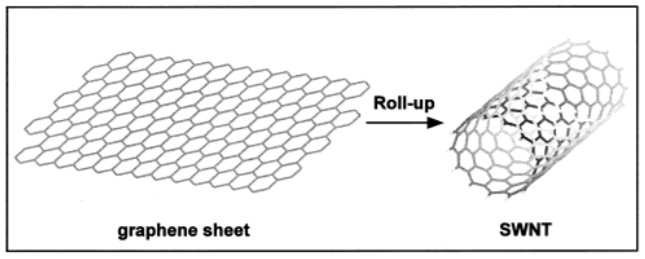
\includegraphics{images/chapter_intro/rolled_up_graphene.png}
	\caption{ Reproduced from \cite{odom2000structure}.}
\end{figure}

Applications in electronic and optoelectronic devices such as transistors, detectors, polarizers, etc. 

The purpose of this thesis focuses on elucidating the ultrafast dynamics of single-wall carbon nanotubes. Previous studies used samples with several different chirlaties, making it harder to distinguish between the dynamics of each chirality. Recent developments have make it possible to make high-purity, single-chirality samples. 

Chapter 2 provides an introduction to the some of the basic properties of carbon nanotubes. Chapter 3 explores prior works ultrafast spectroscopy measurements of carbon nanotubes. Chapter 4 illustrates the relevant experimental procedures. Chapter 5 presents coherent processes that have been observed. Chapter 6 discusses dynamics that occur after pumping above the bandgap.